\documentclass[10pt,twocolumn,a4paper]{article}
\usepackage[margin=0.7in,columnsep=0.25in]{geometry}
\usepackage[T1]{fontenc}
\usepackage[utf8]{inputenc}
\usepackage{lmodern}
\usepackage{microtype}
\usepackage{graphicx}
\usepackage{booktabs}
\usepackage[font=small,labelfont=bf,skip=2pt,justification=raggedright,singlelinecheck=false]{caption}
\usepackage[hidelinks]{hyperref}
\usepackage{titlesec}
\titleformat{\section}{\normalsize\bfseries}{\thesection.}{0.5em}{}
\titlespacing*{\section}{0pt}{5pt}{1pt}
\setlength{\parskip}{1pt}
\renewcommand{\refname}{References}

\title{}
\author{}
\date{}

\begin{document}
\pagestyle{empty}

\begin{center}
{\Large\bfseries Canvas360: Routing Image Edits to Specialised Pipelines\par}
\vspace{3pt}
{\normalsize Shresth Keshari\\[-1pt] \textit{Team B76, IIT Bombay}\par}
\vspace{1pt}
{\small Inter-IIT Tech Meet 14.0, Adobe problem statement}
\end{center}

\begin{abstract}
\noindent Generative image editors are reliable on broad requests but often fail on edits that need identity preservation, restraint, or physical consistency. We present Canvas360, a prototype that treats editing as intent routing. A Flan-T5 classifier maps each prompt to one of five intents, and the request goes to the cheapest pipeline that can serve it: semantic colour grading, structure-locked stylisation, general instruction editing, a draft-critique-refine remix loop, or manual tools. On hot runs, colour grading takes about 0.90\,s and stylisation 7.4--9.1\,s. One logged general edit takes 242.6\,s. The repository contains a Tkinter editor with a local language-model command parser and a SAM~2 segmentation wrapper. The generative pipelines are described but their code is not included. No human-preference or identity-similarity evaluation was performed.
\end{abstract}

\section{Introduction}
Phone-first creators want professional-level edits, but desktop editors are dense, and generative editors are unreliable on the edits people care about most. This paper responds to the Adobe problem statement of Inter-IIT Tech Meet 14.0, which asks how image editing can move from pixel tools toward user intent. We target three failure modes of generative editing: \emph{identity loss}, where a subject changes when only its colour should; \emph{unrequested changes}, such as smoothing skin or relighting the whole frame; and \emph{poor compositing}, where a subject moved into a new scene floats under mismatched light. Taesiri et al.~\cite{taesiri2025} study how generative AI tools handle everyday editing requests, which motivates judging editors on concrete tasks. Our design rule is to \emph{route first, then run the smallest model that fits}: a colour grade should never trigger a diffusion model.

\section{Related Work}
ControlNet~\cite{controlnet} conditions diffusion on edge maps, IP-Adapter~\cite{ipadapter} injects image-prompt features through cross-attention, and SDXL~\cite{sdxl} is the base generator. Qwen-Image-Edit~\cite{qwenimage} handles open-ended text edits, and FLUX.1 [dev]~\cite{flux} is a high-fidelity generator. SAM~2~\cite{sam2} gives promptable masks, Mask2Former~\cite{mask2former} gives panoptic classes, and InternVL3.5~\cite{internvl} serves as a vision-language critic. T2ONet~\cite{t2onet} learns language-guided global edits from FiveK retouching pairs~\cite{fivek}. Flan-T5~\cite{flant5} classifies intents, U\textsuperscript{2}-Net~\cite{u2net} via rembg~\cite{rembg} removes backgrounds, and Llama~3.2~\cite{llama32} is the local command parser.

\section{Method}
\begin{figure}[t]
\centering
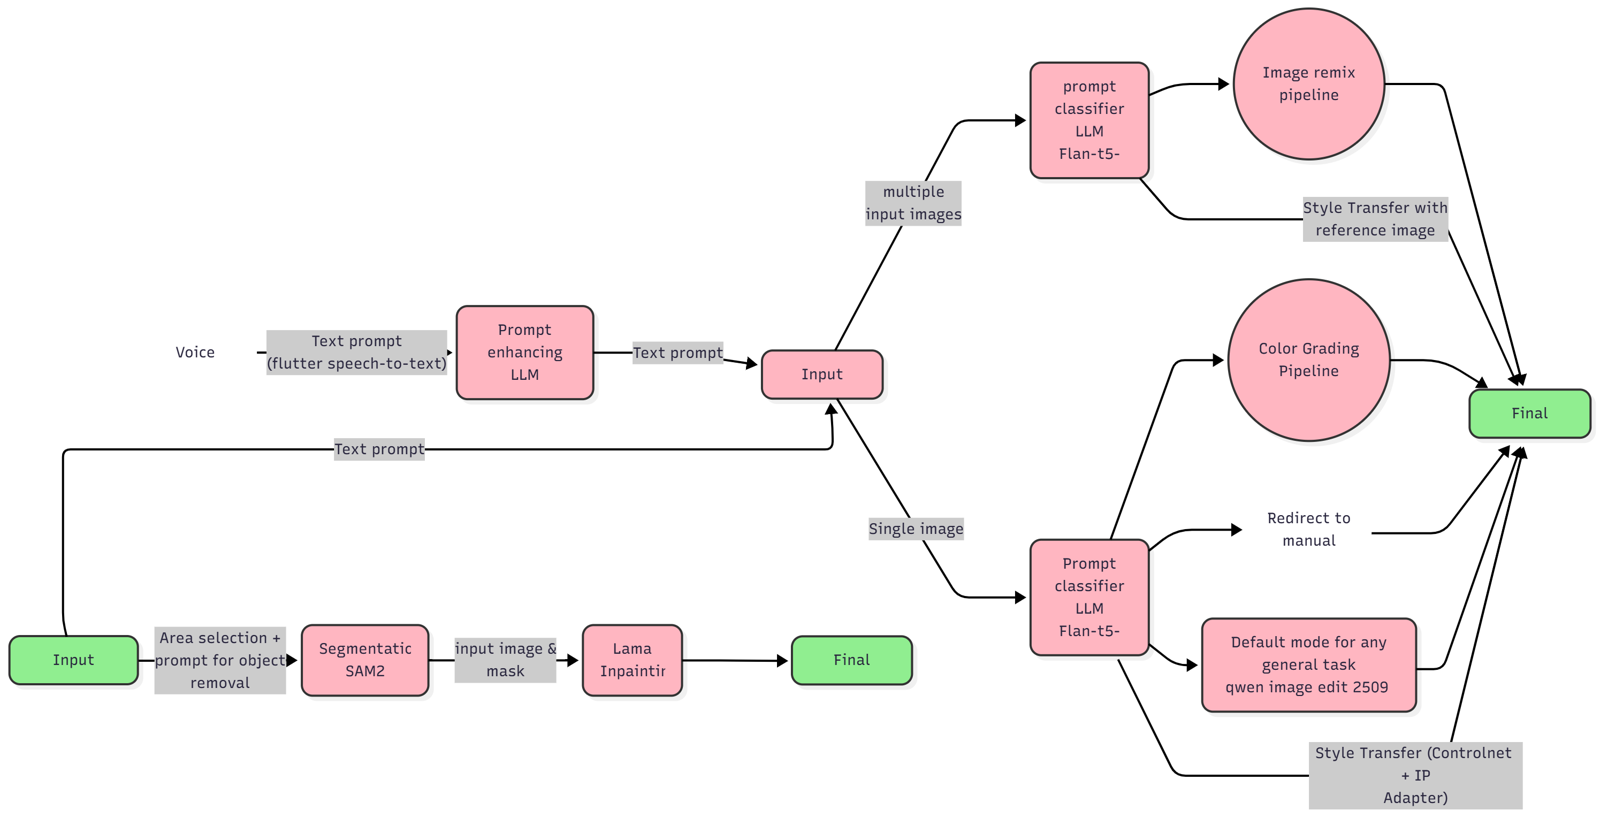
\includegraphics[width=\columnwidth]{../docs/diagrams/main_flow.png}
\caption{Team overview diagram from the repository. The diagram also shows a SAM~2 mask followed by inpainting and a voice-input path; these are not evaluated here and the inpainting code is not in the repository.}
\label{fig:overview}
\end{figure}

\subsection{Routing}
A Flan-T5 router compares the log-probabilities of five intent tokens, \texttt{[STYLE]}, \texttt{[COLOR]}, \texttt{[EDIT]}, \texttt{[MANUAL]} and \texttt{[REMIX]}. Scoring five tokens avoids free-form generation, so routing is one forward pass. Every branch returns a suggestion the user can accept or reject.

\subsection{Pipelines}
\textbf{Semantic colour grading.} Mask2Former, trained on COCO-Panoptic, segments the scene into classes, and a dictionary maps class groups to OpenCV recipes. Vegetation gets a 1.20$\times$ green gain; sky and water get a 0.85$\times$ red reduction and a 1.10$\times$ blue boost.

\textbf{Structure-aware stylisation.} Canny edges of the input go to ControlNet-Canny, which fixes the object's boundaries. An IP-Adapter injects the style of a reference image, or of one SDXL generates from a text prompt. Loading SDXL with ControlNet takes about 40\,s and over 8\,GB of VRAM, so a process-wide cache keeps the models resident. Afterwards rembg (U\textsuperscript{2}-Net) restores the original background.

\textbf{General edit and remix.} The general branch sends open-ended instructions to Qwen-Image-Edit. The remix branch drafts a composite with Qwen-Image-Edit, has InternVL3.5 list physical and lighting faults as action commands, and refines with FLUX.1 [dev]. Manual tools (crop, rotate, brush, filters) call no model.

\textbf{Runnable code.} The local editor (\texttt{src/local\_editor/}) is a Tkinter application in which a quantised Llama~3.2 1B model (Q4\_K\_M GGUF, llama-cpp-python) turns a prompt into a JSON edit command; a keyword-only fallback works without it. The segmentation wrapper (\texttt{src/segmentation/}) exposes point, box and lasso prompts on SAM~2.1 (Hiera-L).

\section{Experiments and Results}
The latency table has no recorded hardware, and each general-edit figure is one run, so none of these numbers is a benchmark.

\begin{table}[h]
\centering
\small
\caption{Hot-run latency (team measurement, hardware not recorded).}
\label{tab:latency}
\begin{tabular}{@{}lr@{}}
\toprule
Task & Hot run \\
\midrule
AI suggestions & $\sim$3.58\,s \\
Prompt classifier & $\sim$2.3--2.9\,s \\
Colour grading & $\sim$0.90\,s \\
Style transfer, reference image & $\sim$7.4\,s \\
Style transfer, text prompt & $\sim$9.1\,s \\
\bottomrule
\end{tabular}
\end{table}

\begin{table}[h]
\centering
\small
\caption{Logged measurements in \texttt{results/metrics/}.}
\label{tab:logs}
\begin{tabular}{@{}l@{\hspace{10pt}}r@{}}
\toprule
Measurement & Value \\
\midrule
Qwen-Image-Edit, inference time (1 run) & 242.6\,s \\
Qwen-Image-Edit, peak VRAM / total & 18.0 / 23.0\,GB \\
T2ONet, val.\ distance at iter.\ 1,000 & 0.1033 \\
T2ONet, best val.\ distance (iter.\ 10,000) & 0.0784 \\
\bottomrule
\end{tabular}
\end{table}

Table~\ref{tab:latency} shows colour grading about eight times faster than reference-image stylisation, and the cache is what keeps the diffusion path in seconds. The 242.6\,s general edit is far from interactive. The T2ONet log is a training record: its metric is undefined in the file, so it is not a comparison with other methods. Qualitative outputs are in \texttt{docs/images/}.

\section{Discussion and Limitations}
\textbf{No quality metric.} Human preference, identity similarity and FID were not computed, so identity preservation is a design rationale, not a measured result. Router accuracy is also unmeasured.

\textbf{Code provenance.} Some pipeline code lived in Google Colab notebooks and is not in this repository. This covers the router, colour-grading, stylisation and remix code, which are described here but not included. The 3D reconstruction code is also absent. Those results are team measurements, not reruns.

\textbf{Timing scope.} Latencies are warm runs on an unrecorded GPU, and the general edit is a single run. The team's feature-scoring matrix and user survey are not reproduced here.

\section{Conclusion}
Canvas360 shows that a cheap classifier can decide which expensive model runs, keeping colour grades fast and generative edits rare. The repository holds the runnable editor, the segmentation wrapper and the logged measurements. Evaluating routing accuracy, output quality and identity preservation is the next step.

\bibliographystyle{unsrt}
\footnotesize
\bibliography{references}

\end{document}
